\documentclass[a4paper,11pt,oneside]{scrreprt}
\usepackage[latin1]{inputenc}
\usepackage[english]{babel}
\usepackage{graphicx}
\usepackage{float}
\usepackage{geometry}
\geometry{verbose,a4paper,tmargin=25mm,bmargin=25mm,lmargin=15mm,rmargin=25mm}
\usepackage{paralist}

\usepackage{paracol}

\usepackage{todonotes}

\usepackage{listings}
\lstset{language=Java,
	tabsize=2,
	showspaces=false,
	showtabs=false,
	breaklines=true,
	showstringspaces=false,
	breakatwhitespace=true,
	commentstyle=\color{pgreen},
	keywordstyle=\color{pblue},
	stringstyle=\color{pred},
	basicstyle=\footnotesize\ttfamily,
	moredelim=[il][\textcolor{pgrey}]{$$},
	moredelim=[is][\textcolor{pgrey}]{\%\%}{\%\%}
}

\usepackage{tikz}
\usetikzlibrary{calc,patterns,angles,quotes}

\usepackage{caption}
\usepackage{subcaption}
\usepackage{tabularx} % in the preamble

\usepackage{pdfpages}

\begin{document}


\begin{center}
	Submitted by Group 51
	
	\bigskip
	
	\begin{tabular}{c}
	Group Members: \\
	CETIN, Ulfet (391819); GRUCZKA, FILIP (413279);	LIPINSKI, Bartosz (413177) \\
	\end{tabular}

	\bigskip
	
	DIS1 WS 19/20 Assignment 4\\
	Types of Knowledge and Mistakes
	
	%	(ordered on lastname basis)
\end{center}

\section*{Task 1}



\vspace{5cm}

\bigskip

\bigskip

\bigskip

\begin{figure}[H]
	\centering 
	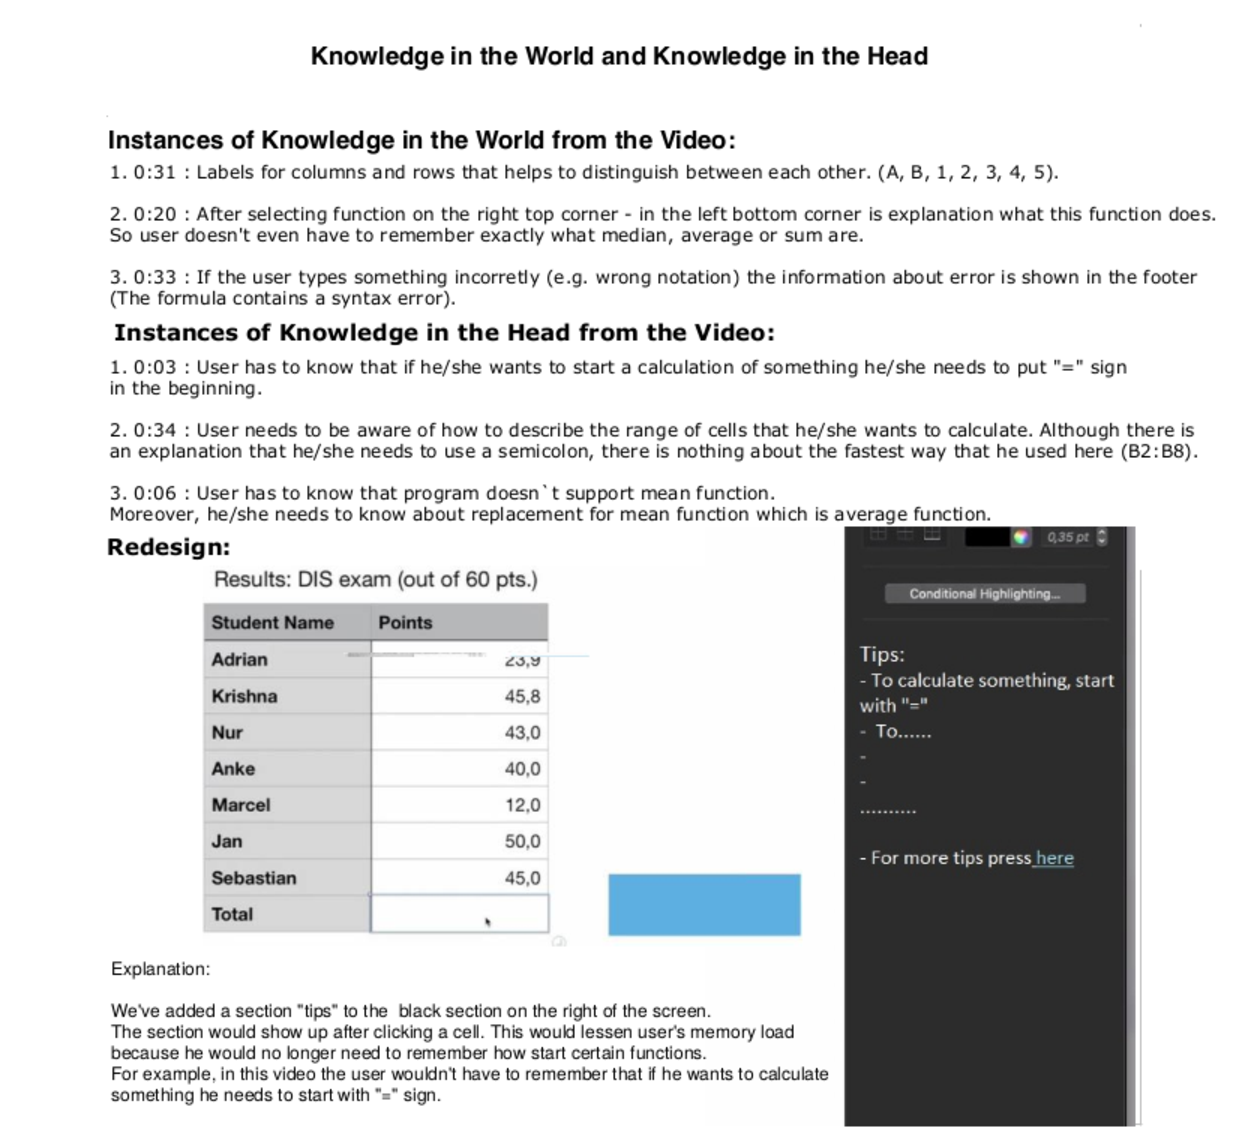
\includepdf[scale=1.0,pages=1-1,clip,trim=0cm 0cm 0cm -4cm, pagecommand={}]{./Q1_resized.pdf}
\end{figure}


\clearpage
\section*{Task 2}



\begin{tabularx}{\textwidth}{|X|}
	\hline
		\textbf{Mistakes}
		\\
	\hline
		\textbf{Task:}
		
		User is requested to change the zoom of the video a zoom value other than the currently set one using the right-click menu of the VLC.
		\\
	\hline
		\textbf{Mistake:}
		
		This is a `\textbf{Rule-based mistake}`, that is, the user evaluates the situation correctly but takes the wrong course of actions.
		
		\\
		
		\textbf{Cause:}
		
		Evaluation: the user oversees the "Always Fit Window" checkbox, and without modifying it, goes ahead to directly change the zoom ratio.
		\\
	\hline
		\textbf{Redesign:}
		
		refer to the picture \ref{fig:sub2} below of this page for the redesign image
		\\
		
		\bigskip
		
		\textbf{Explanation:}
		
			\begin{compactenum}[	a)]
				\item How the redesign minimizes the implications of the mistake:
				
					all the zoom-related buttons and checkboxes are under the same menu
					
					\bigskip				
					
				\item How the redesign minimizes the chances of the mistake occurring in the future:
				
					the user, before clicking on a zoom ratio, would notice the "Always Fit Window" checkbox in the very same submenu, and would think that it is related to zooms, as it should be. Even though the user might fall for this the first time, just like we displayed in our user test, in the subsequent trials, the user can notice this checkbox being in the same submenu, and may decide to play with it too.
			\end{compactenum}
	\\
	\hline
	
	
	
	%	\raisebox{-\height}[0pt][0pt]{
\includegraphics[clip, trim=0cm 0cm 0cm 0cm, scale=0.2]{./images/redesign.png} }
	
	%	\hline
	
\end{tabularx}\\

\begin{figure}[H]
	\centering
	\begin{subfigure}{.5\textwidth}
		\centering
		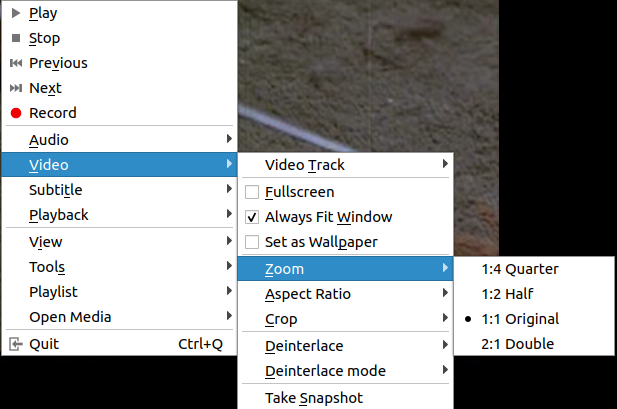
\includegraphics[clip, trim=0cm 0cm 0cm 0cm, scale=0.35]{./images/vlc_original.png}
		\caption{Original}
		\label{fig:sub1}
	\end{subfigure}%
	\begin{subfigure}{.5\textwidth}
		\centering
		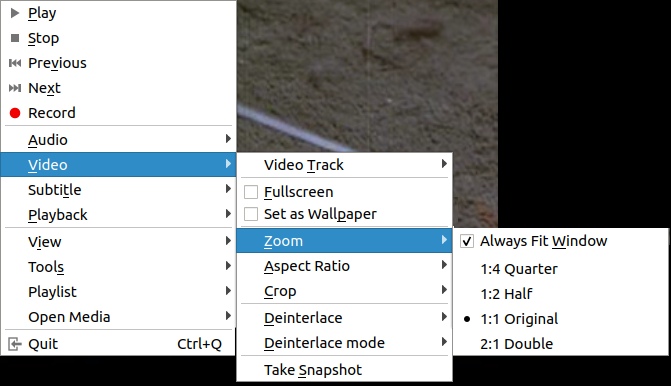
\includegraphics[clip, trim=0cm 0cm 0cm 0cm, scale=0.50]{./images/vlc_redesign.png}
		\caption{Redesign}
		\label{fig:sub2}
	\end{subfigure}
	\caption{Video Lan Client (VLC) Right-Click Menu}
	\label{fig:test}
\end{figure}

\end{document}}
